\documentclass[sigconf]{acmart}

\usepackage[english]{babel}
\usepackage{blindtext}

% Copyright
\renewcommand\footnotetextcopyrightpermission[1]{} % removes footnote with conference info
\setcopyright{none}
%\setcopyright{acmcopyright}
%\setcopyright{acmlicensed}
%\setcopyright{rightsretained}
%\setcopyright{usgov}
%\setcopyright{usgovmixed}
%\setcopyright{cagov}
%\setcopyright{cagovmixed}

\settopmatter{printacmref=false, printccs=false, printfolios=true}

% DOI
\acmDOI{}

% ISBN
\acmISBN{}

%Conference
%\acmConference[Submitted for review to SIGCOMM]{}
%\acmYear{2018}
%\copyrightyear{}

%% {} with no args suppresses printing of the price
\acmPrice{}
\usepackage[linesnumbered, boxed]{algorithm2e}
\usepackage{multirow}
\usepackage{subfigure}
\usepackage{tikz}
\usetikzlibrary{calc,trees,positioning,arrows,chains,shapes.geometric,decorations.pathreplacing,decorations.pathmorphing,shapes,matrix,shapes.symbols}
\DeclareMathOperator*{\argmax}{arg\,max}
\DeclareMathOperator*{\argmin}{arg\,min}
\begin{document}
\title{Traffic-aware topology design using Lagrangian Duality Theory}

%\titlenote{Produces the permission block, and copyright information}
%\subtitle{Extended Abstract}

\author{Min Yee Teh, Shizhen Zhao}
% \author{Firstname Lastname}
% \authornote{Note}
% \orcid{1234-5678-9012}
% \affiliation{%
%   \institution{Affiliation}
%   \streetaddress{Address}
%   \city{City} 
%   \state{State} 
%   \postcode{Zipcode}
% }
% \email{email@domain.com}

% The default list of authors is too long for headers}
\renewcommand{\shortauthors}{Teh .et al.}

\begin{abstract}
    \blindtext
\end{abstract}

\maketitle

\newcommand{\floor}[1]{\left\lfloor #1 \right\rfloor}
\newcommand{\ceil}[1]{\left\lceil #1 \right\rceil}
\section{Introduction}

The wealth of applications that run on data centers today has brought about irregular traffic patterns, which have confounded data center networking design for a long time. Recent literature have suggested that this wealth of application variety leads to inter-rack traffic patterns that are highly non-uniform \cite{benson2010network, benson2009understanding}. This implies a high degree of traffic locality, and that all-to-all traffic do not arise as frequently as most would assume. This traffic asymmetry is projected to increase in the future as more applications are run on the cloud. What is most surprising is that while there is a general consensus within the data center community on the unpredictability and transient burstiness of inter-rack traffic, studies [9] have found that the traffic locality can persist over a period of months or more. 

One way to ''even'' non-uniform traffic patterns is to load-balance using workload migration \cite{jain2012topology}. However, as data center tends towards disaggregated hardware resources \cite{papaioannou2016benefits}, relying solely on workload placement and migration will become increasingly difficult, since resource disaggregation of compute elements and storage elements will force same workloads to be mapped to physically-separated clusters. Careful job placement even with global knowledge cannot fundamentally even out the strong pairwise traffic pattern generated due to desegregation. Another solution to even-ing out non-uniform traffic is through the use of congestion-aware routing schemes. However, all these routing schemes require traffic flow to be deflected non-minimally to less congested areas first. This adds to the total network traffic and can often create previously unforeseen hotspots in other network areas. We therefore believe that load-balancing through simply intelligent routing or workload placement cannot sufficiently decongest the network under non-uniform traffic permutations. 

To address the non-uniform traffic demands, dynamically-reconfigurable topologies like the Firefly \cite{hamedazimi2014firefly} and ProjectTor \cite{ghobadi2016projector} have been proposed using revolutionary hardware, both of which involve wireless solutions using free space optics. These topologies rely heavily on novel hardware architectures that are immature and difficult to control, as free space optics require highly precise laser-to-detector alignment that is prone to failure. The switching time for these fabrics are shown to be on the order of 10`s of microseconds, allowing them to in theory react to transient traffic bursts. However, our findings show that the topology need not be reconfigured frequently, since we've observed that the majority of inter-rack traffic flows are long-lived (on the order of weeks), an observation also shared by Delimitrou et al \cite{delimitrou2012echo}. This observation has led us to believe that a topology reconfigurable on the order of weeks can still significantly improve network performance by serving the long-lived traffic flows.

We propose a traffic-aware topology built using robust and commercially-available technologies that are already deployed in today's data centers \cite{zhao2018minimal}. More specifically, we've decided to restrict our fabric design to topologies within the direct connect topology family due to their cost effectiveness and high-bisection bandwidth \cite{radhakrishnan2013dahu}. To accommodate the incremental growth and need to alter topology based on long-term traffic patterns, we interconnect the server blocks using a layer of patch-panel. Although patch-panels cannot be rapidly reconfigured to serve transient traffic bursts, our production traffic have shown that on a large timescale, traffic patterns do not change much. Our results further show that simply reconfiguring the patch-panel on a monthly-basis is sufficient in increasing network throughput. 

While the idea of a traffic-aware reconfigurable topology is simple, finding the optimal solution presents a formidable algorithmic challenge. To facilitate understanding, it is convenient to think of this as a supply-demand matching problem, with inter-rack links being the supply and traffic flows being the demand in our case. Within theoretical computer science, this problem can be mapped onto a multicommodity-flow problem, which is NP-hard \cite{irving1994three, foerster2018characterizing}. This problem presents a significant combinatorics challenge due to the coupling of network links introduced through the physical topology constraints, i.e links cannot be formed if they are not connected to the same patch-panel. To our knowledge, no literature on dynamic topology to date have treated this problem rigorously while accounting for physical constraints, with most published work resorting to immature hardware technologies \cite{hamedazimi2014firefly, ghobadi2016projector} to circumvent this problem. Yet finding a solution to this problem is crucial for the deployment of traffic-aware topologies within data centers currently in-production.

Hence, our main contribution in this work is the design of a robust and scalable polynomial time topology-design methodology based on predicted traffic pattern, while taking into account constraints imposed by the physical connectivity. We include this constraint in our problem formulation without reverting to an ILP formulation, and propose a 2-step algorithm to decompose this problem into more manageable subproblems. The first step involves finding an optimal fractional topology which minimizes maximum link utilization under a given traffic load. Using this step, we derive the optimal fractional connectivity between different server blocks, which can be solved quickly using a linear program. Subsequently, we attempt to ''match'' the topology`s connectivity with the optimal fractional connectivity using convex optimization \cite{low1999optimization}. Using this technique, we show that our integer connectivity matches the optimal fractional topology very closely, without resorting to solving complex integer-linear programs.

Finally, we simulate the effectiveness of our methodology using different metrics across several heterogeneous data center fabrics. Through our simulation results, we show that reconfiguring a topology once a month is enough to lower maximum link utilization by as much as $20\%$. We further show that our methodology minimizes total network traffic by reducing the average hop count of flows, lowering average link utilization by as much as $50\%$. Furthermore, our analysis shows that topology engineering also significantly lowers the percentile link utilizations, keeping about $50\%$ of the network links idle under most load conditions. Most importantly, our methodology allows us to achieve all these metrics using only about half the network links, giving us a $2\times$ economic saving on network resources without sacrificing network throughput. 

\begin{figure*}[h]
\centering
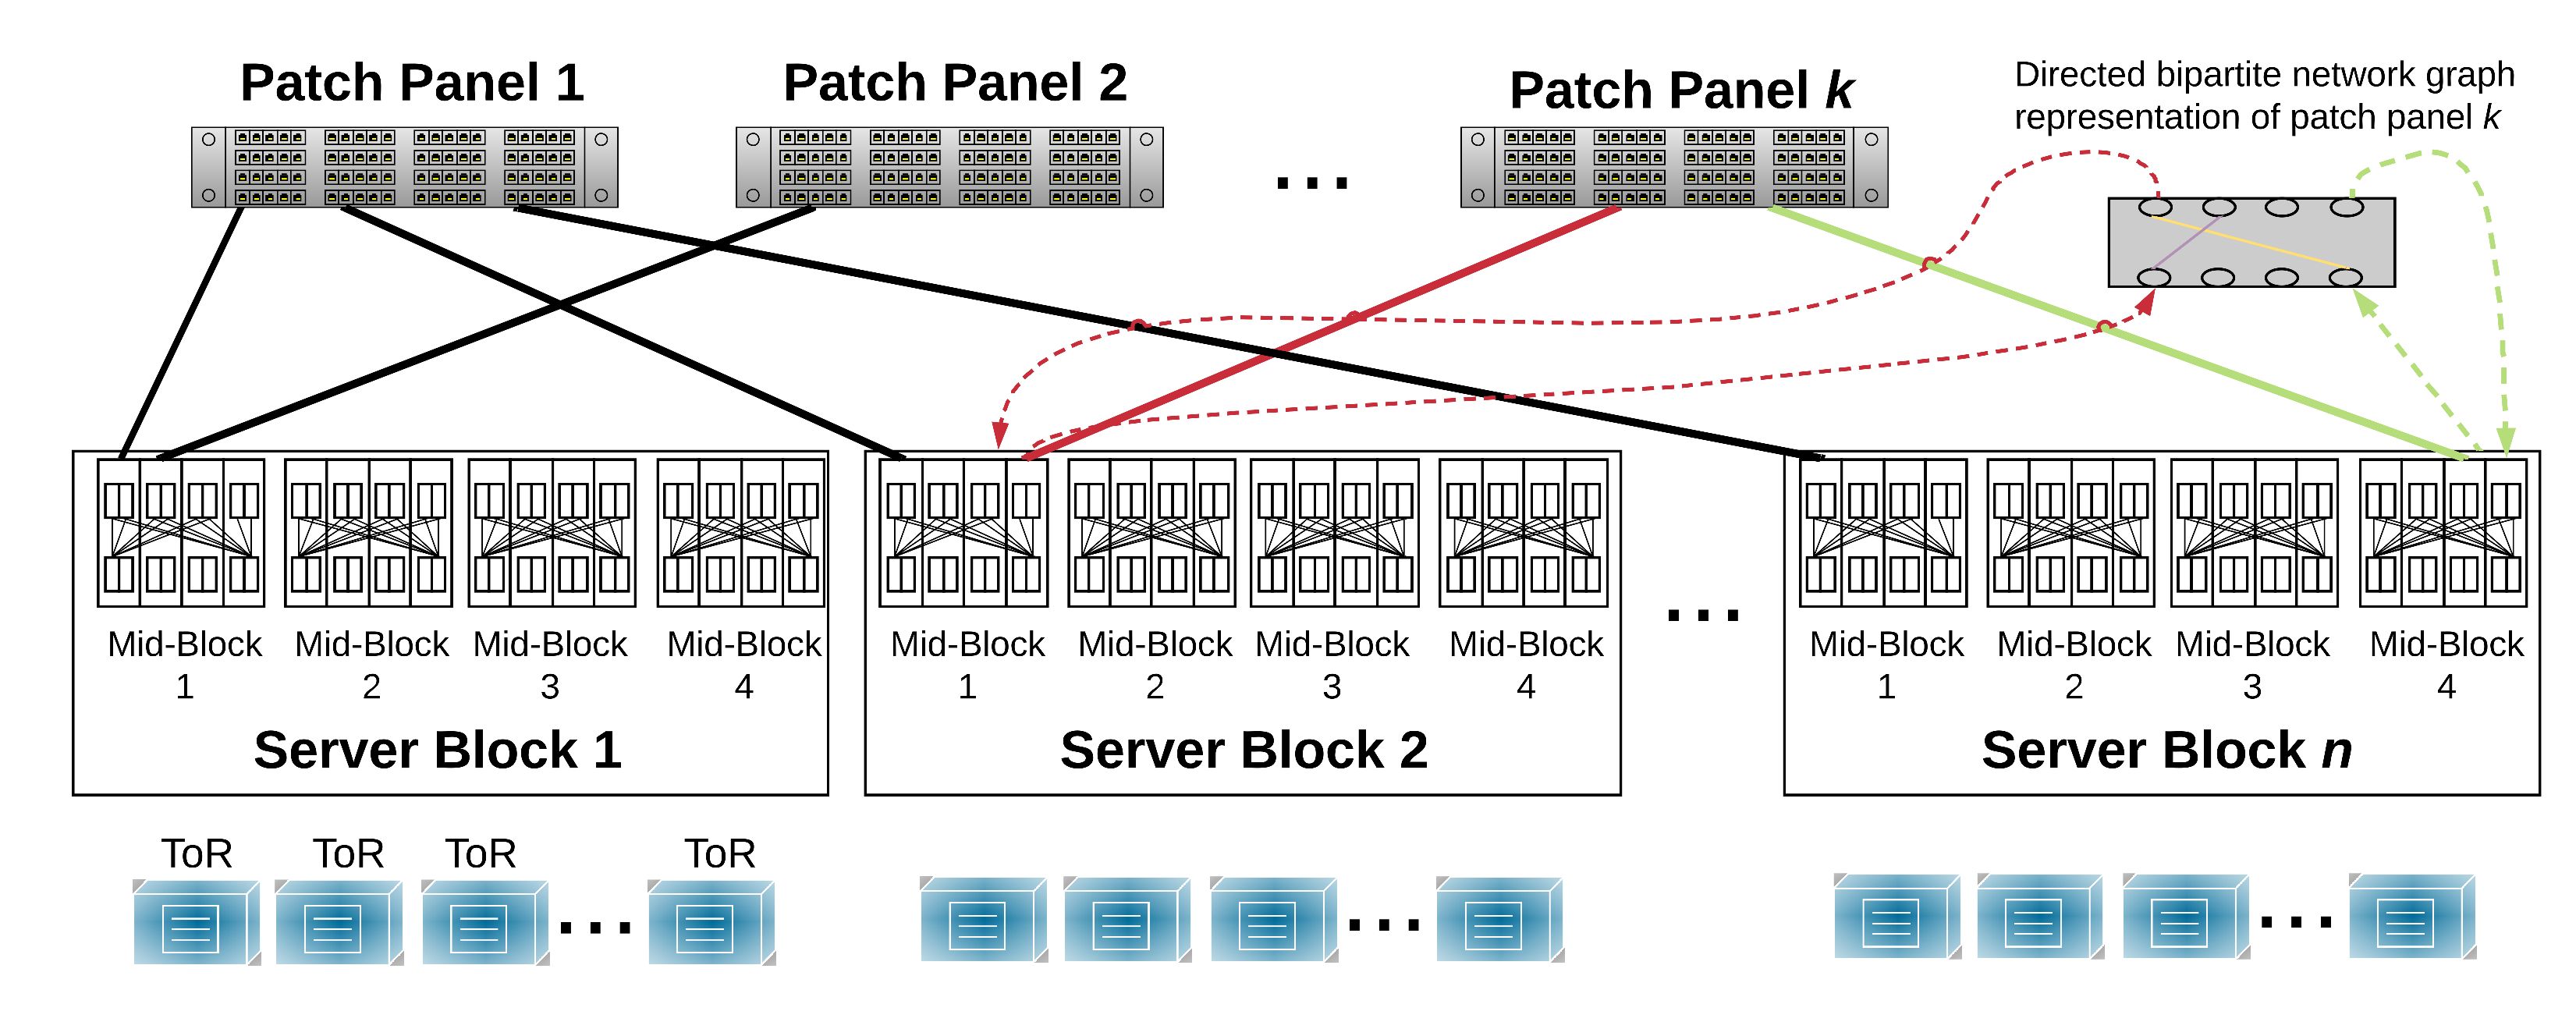
\includegraphics[width=\textwidth, scale=0.55]{./figures/topology.eps}\label{direct_connect_topology}
\caption{Direct-connect topology interconnected via a patch-panel layer, alongside an illustration on the bipartite network graph representation of patch-panel \textit{k}. All links in solid lines are bidirectional (undirected), while dotted links of the same color are the unidirectional (directed) representation of the same solid link.}
\end{figure*}

\section{Related Work}

In the field of data center topologies, several novel, non-traffic aware topologies have been proposed using a graph-theoretic approach, such as Jellyfish \cite{singla2012jellyfish} and Xpander \cite{valadarsky2015xpander} that are based on random-regular graphs and expander graphs, respectively. These topologies cannot be designed to best cater to the non-uniform traffic that often arise in modern data centers. Although both Jellyfish and Xpander offer excellent incremental expandability, they do not guarantee network diameter as network expands, rendering them suboptimal when running latency-sensitive applications. 

Some literature have suggested hybrid topologies \cite{liu2015scheduling, farrington2011helios} to alleviate network hotspots, with the central idea being the electrical network forming the reliable backbone and route mice flows, while using optical reconfigurable circuits to opportunistically route elephant flows. However, these topologies can be expensive to build due to their hybrid architecture presenting significant hardware engineering challenges, which further delays their widespread use in today's data centers. Others dynamic topologies like ProjectTor \cite{ghobadi2016projector} proposes a ''disco ball'' device that reconfigures ToR switches by changing mirrors to reflect different laser emissions unto different photodiode receivers. This presents a single point of failure, since a slight misalignment of the disco ball can potentially disconnect the entire data center fabric. FireFly \cite{hamedazimi2014firefly} proposes attaching laser sources and photodiode receivers to each ToR and forming interrack links using a ceiling mirror for deflection, with each interrack link being a lightpath between the source ToR and destination ToR. Both papers proposed mirror-reconfiguring algorithm that assume any arbitrary link on a source ToR switch can reach at least one receiver on the destination ToR. This assumption is highly unrealistic in wired networks since links connected to different switches being unconnectable. 

Dynamic topologies have also seen its debut in the HPC community through the Flexfly topology \cite{wen2016flexfly}, which is based on a Dragonfly topology reconfigures its intergroup links using silicon-photonic optical switches. While Flexfly offers immensely short switching time, the algorithm proposed by the author(s) requires examining number of switch states, which grows exponentially with the number of ports in the optical switch. As such, employing the proposed algorithm in any deployed data centers of reasonable size infeasible. In addition, the paper also acknowledges that increasing portcount in silicon photonic switches is technologically-challenging, and therefore severely limiting its ability to be integrated into current high-radix data center fabrics. 



\section{Definitions and Notations}
In order to rigorously formulate the network reconfiguration problem, we begin by introducing a series of useful notations and definitions.

%% include the table of notations here

\begin{table}
\begin{tabular}{|p{1.7cm}|p{6.5cm}|}
\hline
$S_i, O_k$ & Server block $i$, patch-panel $k$ \\
\hline
$\eta$ & Max link utilization \\
\hline
$c_{ij}$ & Maximum possible bandwidth capacity between $S_i$ and $S_j$\\
\hline
$x_{ij}^k$ & Number of server block $i$'s northports connected to server block $j$'s southports through patch-panel $k$ \\ 
\hline
$D \in \mathbb{R}^{n\times n}$ & Demand matrix, used interchangeably with the optimal fractional topology\\ 
\hline
$l_n^k(S_i), l_s^k(S_j)$ & Number of physical links connecting $S_i$ to northport of $O_k$, and $S_j$ to southport of $O_k$, respectively\\
\hline
$P_k(S_i, S_j)$ & Number of port-disjoint paths leading from $S_i$ to $S_j$ via $O_k$. Therefore, $L_k(S_i, S_j) = \min(l_n^k(S_i), l_s^k(S_j))$\\
\hline
$U_{ij}^k(x_{ij}^k)$ & Primal problem's objective function element, generally referring to $- (x_{ij}^k - \min(l_n^k(S_i), l_s^k(S_j)))^2$ \\
\hline
$\phi^+$ & $\phi^+ = \max(0, \phi)$ \\
\hline
\end{tabular}
\caption{Commonly-used notations} 
\label{notations}
\end{table}

\begin{itemize}
\vspace{-4pt}
    \item \textbf{Physical Topology} Describes the physical connectivity between the server blocks and the patch panels within the network, and can be represented as a directed graph.
    \item \textbf{Logical Topology} Describes the connectivity between server blocks, abstracting away the layer of patch-panels.
    \item \textbf{Fractional Topology} The logical topology assuming that link counts between server blocks can occupy non-integer values. 
    \item \textbf{Southports, Northports} Southports refer to patch-panel outgoing ports, with an outgoing (south-facing) link towards server blocks. Northports on the other hand are connected to incoming (north-facing) links incident on server blocks.
\end{itemize}
We assume each patch panel can be represented as a bipartite network flow graph, as shown in Figure \ref{direct_connect_topology}. Each bidirectional link are modeled as two directed links, . It turns out, modeling the topology as a directed graph possesses a a key mathematical importance, since our patch-panel reconfiguration methodology does not need to impose the constraint of $x_{ij}^k = x_{ji}^k$ for any $i \neq j$. 

\section{Traffic-aware Topology-Design}
\subsection{Demonstrating Traffic-aware Topology Design Benefits}
We consider 2-hop routing so as to allow some the network to load-balance through routing. Consider the following example:

%%Draw the 4 point graph and dummy example with mlu improvement by 50% with topology engineering, and claim that it generalizes to varying degrees of improvement for M-to-N bipartite communications

We posit that there are certain traffic patterns under which traffic-aware topology design will prove most useful. One such example is a $M$-to-$N$ bipartite traffic pattern, whereby each of the $M$ senders send traffic to all $N$ receivers. These traffic are expected to arise when datacenter architectures become increasingly disaggregated, where there are $M$ compute server blocks that need to write data into storage distributed across $N$ storage blocks. To clarify this concept, we present the following example:\\\\
Consider a datacenter network with 2 sets of server blocks $A = \{a_1, a_2, ..., a_n\}$ and $B = \{b_1, b_2, ... , b_n\}$, whereby the set of all server blocks is given as $S = A \cup B$. The network topology is that of an all-to-all with a uniform link capacity of $c$. Suppose we have the traffic demand described by:
\begin{equation}
\begin{aligned}
    T(a_i, b_j) = \begin{cases}
                \alpha, \text{ if } a_i \in A \text{ and } b_j \in B\\
                0, \text{ otherwise}
    \end{cases}
\end{aligned}
\end{equation}
We assume 2-hop routing for network load-balancing, and every node can be used as an intermediate hop. Using the available uniform topology shown in Figure \ref{uniform_topology}, the max link utilization with perfect load balancing is $\frac{(2n-1)\alpha}{c}$. Using traffic-aware topology design, however, we can disconnect the $n - 1$ links that each sender in $A$ to other sender nodes in the same set, and connect them to $n - 1$ receivers in set $B$ instead, resulting in the topology shown in Figure \ref{traffic_aware_topology}. In this case, the max link utilization under perfect load-balancing is $\frac{n \alpha}{c}$. This shows that with traffic-aware topology designs we can reduce max link utilization to a factor of $\frac{n}{2n - 1} \approx \frac{1}{2}$ than that obtained form traffic-agnostic topologies.
\begin{itemize} 
    \item \textbf{Singular hotspot} - When there is a singular hotspot, the most congested links will be either the egress or ingress links of the hottest block. Under these traffic conditions, max link utilization (MLU) cannot be driven down through intelligent topology design, as the congestion is attributed to the server block's physical ability to pushing traffic out or in.
    \item \textbf{Uniform traffic} - Under a uniform traffic load, there is no need for special topology design. The ideal topology to handle a uniform traffic pattern will be to uniformly connect all the server blocks within the topology.
\end{itemize}

\begin{tikzpicture}[->,>=stealth',shorten >=1pt,auto,node distance=2cm,
                    thick,main node/.style={circle,draw,font=\sffamily\Small\bfseries}]
  \node[main node] (1) {$a_1$};
  \node[main node] (2) [right of=1] {$a_2$};
  \node[main node] (3) [right of=2] {$a_3$};
  \node[main node] (4) [right of= 3, xshift=1cm] {$a_n$};
  \node[main node] (5) [below of=1] {$b_1$};
  \node[main node] (6) [below of=2] {$b_2$};
  \node[main node] (7) [below of=3] {$b_3$};
  \node[main node] (8) [below of=4] {$b_n$};
  
  \node at ($(3)!.5!(4)$) {\ldots\ldots};
  \node at ($(7)!.5!(8)$) {\ldots\ldots};
  
  \path[every node/.style={font=\sffamily\small}]
    (1) edge node [left] {$c$} (5)
        edge node[left] {} (6)
        edge node [left] {} (7)
        edge node [left] {} (8)
        edge node [-] {} (2)
        edge [bend left] node [bend left] {} (3)
        edge [bend left] node [left] {$c$} (4)
    (2) edge node [left] {} (5)
        edge node [left] {} (6)
        edge node [left] {} (7)
        edge node [left] {} (8)
    (3) edge node [right] {} (6)
        edge node [right] {} (7)
    (4) edge node [right] {} (6)
        edge node [left] {} (5);
\label{uniform_topology}
\end{tikzpicture}


\begin{tikzpicture}[->,>=stealth',shorten >=1pt,auto,node distance=2cm,
                    thick,main node/.style={circle,draw,font=\sffamily\Small\bfseries}]
  \node[main node] (1) {$a_1$};
  \node[main node] (2) [right of=1] {$a_2$};
  \node[main node] (3) [right of=2] {$a_3$};
  \node[main node] (4) [right of= 3, xshift=1cm] {$a_n$};
  \node[main node] (5) [below of=1] {$b_1$};
  \node[main node] (6) [below of=2] {$b_2$};
  \node[main node] (7) [below of=3] {$b_3$};
  \node[main node] (8) [below of=4] {$b_n$};
  
  \node at ($(3)!.5!(4)$) {\ldots\ldots};
  \node at ($(7)!.5!(8)$) {\ldots\ldots};
  
  \path[every node/.style={font=\sffamily\small}]
    (1) edge node [left] {$2c$} (5)
        edge node[left] {} (6)
        edge node [left] {} (7)
        edge node [left] {} (8)
    (2) edge node [left] {} (5)
        edge node [left] {} (6)
        edge node [left] {} (7)
        edge node [left] {} (8)
    (3) edge node [right] {} (6)
        edge node [right] {} (7)
    (4) edge node [right] {} (6)
        edge node [left] {} (5);
\label{bipartite_traffic}
\end{tikzpicture}


Assuming that every link has capacity $c$, and 

\subsection{Deriving the Optimal Fractional Topology}
We employ a 2-hop routing scheme to allow for better load-balancing across the network links. Our goal is to minimize the max link utilization under a given traffic load. This can be formulated as a linear program that can be solved easily and quickly. 
\begin{equation}\label{fractional_graph}
\begin{aligned}
\min \;& \quad \eta \\
\text{s. t: } & 1) \sum_{j \in S \backslash \{i\}} d_{ij} \leq a_i \quad \forall \; i \in S\\
& 2) \sum_{i \in S \backslash \{j\}} d_{ij} \leq a_j \quad \forall \; j \in S \\
& 3) \; \omega_{ij} + \sum_{k \in S \backslash \{i, j\}} \omega_{ij}^k = t_{ij}, \quad \forall \; i, j \in S \\
& 4) \sum_{k \in S \backslash \{i, j\}} \omega_{kj}^i  + \sum_{k \in S \backslash \{i, j\}} \omega_{ik}^j + \omega_{ij} \leq \eta \; d_{ij} b_{ij}, \forall i, j \in S
\end{aligned}
\end{equation}
Where $b_{ij} = \min(b_i, b_j)$. Constraints 1 and 2 denote the physical outgoing and incoming link counts. Constraint 3 enforces the rule that all traffic from source $i$ to destination $j$ must be flown through either 1 or 2 hops through an intermediate superblock. Constraint 4 then enforces all link utilizations to be at most equal to that of the max link utilization. The derived fractional topology then acts as a demand matrix for the next matching step.

%% Point 1: mention 2-hop routing
%% Introduce the 

\subsection{Matching the Optimal Fractional Topology}
Given a demand matrix, $D$, we attempt to match the logical topology with that of the demands, subject to physical constraints and connectivity constraints.
\subsubsection{Primal Problem}
\textbf{\\Physical Constraints: } This constraint states that the total number of integral flows that reach $S_j$ through $O_k$ cannot exceed the total physical links connecting the southports of $O_k$ to $S_j$:
\begin{equation}\label{phy_constraint1}
    \sum_{i \in S} x_{ij}^k \leq l_s^k(j) \quad \forall \; k \in O, j \in S
\end{equation}
By reciprocity, total number of integral flows through $O_k$ originating from $S_i$ cannot exceed the total number of physical links connecting the northports of $O_k$ to $S_i$.
\begin{equation}\label{phy_constraint2}
    \sum_{j \in S} x_{ij}^k \leq l_n^k(i) \quad \forall \; k \in O, i \in S
\end{equation}
\textbf{Connectivity Constraints: } In addition to the physical constraints, we also want to ''match'' the logical topology with the fractional topology. We do this by introducing the following constraint:
\begin{equation}\label{con_constraint}
    c_{ij}^L \leq \sum_{k \in O} x_{ij}^k \leq c_{ij}^U, \quad \forall \; i,j \in S
\end{equation}
Where $d_{ij}$ is the fractional link count between $S_i$ and $S_j$, $c_{ij}^L = \floor{d_{ij}}$ and $c_{ij}^U = \floor{d_{ij}}$. Constraint (\ref{con_constraint}) allows us to obtain a logical topology with link counts that are the closest integers to the optimal demand. \\
\textbf{Primal Objective Function: } %% talk more about the primal problem's objective function
\begin{equation}\label{primal_objective}
\begin{aligned}
    \mathbf{P: } & \max_{d_{ij}^k} \sum_{k \in O}\sum_{i, j \in S}U_{ij}^k(d^k_{ij})\\
     \text{subject} & \text{ to: } \quad (\ref{phy_constraint1}), \; (\ref{phy_constraint2}), \; (\ref{con_constraint})\\
\end{aligned}
\end{equation}
Special care much be given in picking a objective function, as a good objective function affects not just the quality of the solution, but should also offer meaningful physical interpretation. With this in mind, we propose a concave objective function that would maximize the formation of logical links.
\begin{equation}\label{primalU}
U_{ij}^k(x_{ij}^k) = - (x_{ij}^k \; - \; P_k(S_i, S_j))^2
\end{equation}
We take advantage of the fact that $L_k(S_i, S_j) \geq x_{ij}^k$ given in constraints (\ref{phy_constraint1}) and (\ref{phy_constraint2}) to ensure that the optimal solution maximizes the utilization of physical links. The concavity of (\ref{primalU}) also helps remove the problem of obtaining suboptimal solutions due getting trapped in a local extremum. \\%Proof???
Solving (\ref{primal_objective}) up front while enforcing integral constraints is provably NP-hard \cite{foerster2018characterizing}, which can be attributed to the coupling of $x_{ij}^k$ variables through constraints (\ref{phy_constraint1})-(\ref{con_constraint}). Ideally, we would be able to rewrite (\ref{primal_objective}) in a way that allows us to separate the optimization variables, and solving a collection of smaller problems instead. To this end, we introduce the dual problem, $D$ to  (\ref{primal_objective}). 

\subsubsection{Dual Problem}\text{\\}
\\Our proposed dual problem is a Lagrangian dual, as inspired by \cite{low1999optimization}, which can be written as follows:
\begin{equation}\label{dual_problem}
\begin{aligned}
    \mathbf{D: } & \min_{p_{ij}^+, p_{ij}^-}\max_{x_{ij}^k \in \Lambda} L(x_{ij}^k, p_{ij}^+, p_{ij}^-)\\
    \text{s.t } & \quad p_{ij}^+ \geq 0, \; p_{ij}^- \geq 0
\end{aligned}
\end{equation}
Where $L(x_{ij}^k, p_{ij}^+, p_{ij}^-)$ denotes the Lagrangian of (\ref{primal_objective}), and $p_{ij}^+, p_{ij}^-$ are the dual variables/Lagrange multiplier terms. The objective function for $\mathbf{D}$ is a maximization problem which we shall denote as $B(x_{ij}^k) = \max_{x_{ij}^k \in \Lambda} L(x_{ij}^k, p_{ij}^+, p_{ij}^-)$. The Lagrangian can be written as:
\begin{equation}\label{lagrangian}
\begin{aligned}
    L(x_{ij}^k, p_{ij}^+, p_{ij}^-) & = \sum_{k \in O}\sum_{i, j \in S}U_{ij}^k(x_{ij}^k) - \sum_{i, j \in S} p_{ij}^+( - c_{ij}^U + \sum_{k \in O}x_{ij}^k) \; + \\
    & \quad \sum_{i, j \in S}p_{ij}^-(- c_{ij}^L + \sum_{k \in O} x_{ij}^k ) 
\end{aligned}
\end{equation}
Plugging (\ref{primalU}) into (\ref{lagrangian}) and rearranging the equation terms helps us arrive at the dual objective function:
\begin{equation}\label{dual_objective}
\begin{aligned}
    B(x_{ij}^k) & = \max_{x_{ij}^k \in \Lambda} \; [\sum_{k \in O}\sum_{i,j \in S} -(x_{ij} - P_{ij}(S_i, S_j))^2 \;\; - \\
    & \; \sum_{i, j \in S} p_{ij}^+(\sum_{k \in O}x_{ij}^k - c_{ij}^U) \; + \; \sum_{i, j \in S}p_{ij}^-(\sum_{k \in O} x_{ij}^k - c_{ij}^L)] \\
    & = -\sum_{k \in O}\min_{x_{ij}^k \in \Lambda} \; [\sum_{i, j \in S} (p_{ij}^+ - p_{ij}^-)x_{ij}^k + (x_{ij}^k)^2] \quad + \\
    & \quad \sum_{i, j \in S} p_{ij}^+ c_{ij}^U \; - \; \sum_{i, j \in S} p_{ij}^- c_{ij}^L \\
    & = \; - \sum_{k \in O} Q_k(x_{ij}^k) \; + \; \sum_{i, j \in S} p_{ij}^+ c_{ij}^U \; - \; \sum_{i, j \in S} p_{ij}^- c_{ij}^L 
\end{aligned}
\end{equation}
Where $Q_k(x_{ij}^k) = \min_{x_{ij}^k \in \Lambda} \sum_{i, j \in S} (p_{ij}^+ - p_{ij}^-)x_{ij}^k + (x_{ij}^k)^2$ is a quadratic program for $O_k$. Note that we've grouped the terms in such a way that the outermost summation is a summation over all of the individual patch-panels in $O$. This allows us to solve $k$ smaller QP's that are much easily-solvable. We've omitted several intermediate steps in (\ref{dual_objective}) for the sake of brevity. Interested readers may find the detailed derivation steps attached in the appendix section.

\subsubsection{Relaxing $Q_k(x_{ij}^k)$'s Integral Constraint}\text{\\}
\\Even after the obtaining a variable decoupling and problem-splitting, solving for $Q_k(x_{ij}^k) \; \forall \; k \in O$ still presents a formidable computation challenge, since we $x_{ij}^k$ have integral requirements. In addition, the number of optimization variables grows as $O(n^2)$, where $n$ is the total number of server blocks, hence rendering a QP highly unsolvable given that our datacenter farbics are rather large, and each patch-panel radix-count numbering in the hundreds. We circumvent this by relaxing the integral constraints, and solving for the following QP: 
\begin{equation}\label{optimal_fractional_ocs_solution}
\hat{x}_{ij}^{k} = \text{argmin}_{x_{ij}^k} \sum_{i, j \in S} (p_{ij}^+ - p_{ij}^-)x_{ij}^k + (x_{ij}^k)^2
\end{equation}
Note that $\hat{x}_{ij}^{k} \in \mathbb{R}$, and are in general not integers. To attain the integer values for $Q_k(x_{ij}^k)$, we perform a Taylor series expansion to linearize $Q_k(x_{ij}^k)$ with respect to $x_{ij}^k$. Doing so allows us arrive at the following approximation for the quadratic program:
\begin{equation}\label{min_cost_flow}
    Q_{k}(x_{ij}^k) \approx \min_{x_{ij}^k \in \Lambda} \sum_{i, j \in S} [(p_{ij}^+ - p_{ij}^-)+ 2(\hat{x}_{ij}^{k})] x_{ij}^k
\end{equation}
This Taylor expansion is necessary as it allows us to approximate the QP with integer constraints with an LP with integer constraints. At this point, solving for \ref{min_cost_flow} is very simple, since it is simply a Minimal-Cost (min-cost) Flow problem, with $(p_{ij}^+ - p_{ij}^-)+ 2(\hat{x}_{ij}^k)$ acting as the cost per unit flow through an arc connecting $S_i$ to $S_j$. This can be easily solved using polynomial-time network flow algorithms like Edmonds-Karp. It is also known that these algorithms will always yield an integer solution, if such a solution indeed exists.

\subsection{Overall Methodology}
In this section, we will deliver the overall algorithm that combines all the individual patch-panel optimization problems into one coherent methodology that solves for the demand-matching problem. This requires us to solve the dual problem of the form (\ref{dual_problem}), which has a concave objective function. To solve this, we propose employing an iterative, gradient-projection based solution to force the convergence of solution to the final, optimal solution. Given the concave nature of (\ref{dual_objective}), there exists only one global optima w.r.t $p_{ij}^+$ and $p_{ij}^-$. In each iteration, the equation that governs the dual variable values for the next iteration can be written as:
\begin{equation}\label{gradient_projection}
\begin{aligned}
p_{ij}^{+}(t + 1) &= p_{ij}^{+}(t) \; - \; \delta \frac{\partial L(x_{ij}^k, \; p_{ij}^{+})}{\partial p_{ij}^{+}}\\
&= p_{ij}^{+}(t) \; - \; \delta (c_{ij}^U - \sum_{k \in O}x_{ij}^k) \\
p_{ij}^{-}(t + 1) &= p_{ij}^{-}(t) \; - \; \delta \frac{\partial L(x_{ij}^k, \; p_{ij}^{-})}{\partial p_{ij}^{-}}\\
&= p_{ij}^{-}(t) \; - \; \delta (- c_{ij}^L + \sum_{k \in O}x_{ij}^k) \\
\end{aligned}
\end{equation}
(\ref{gradient_projection}) seems implies that the dual variables are updated every iteration. This formulation has a serious in that for each iteration, all the patch-panels which share the same physical striping will end up being configured the same way. As a result, the solutions for (\ref{dual_problem}) becomes highly oscillatory. We require a formulation of the dual variables that allows for more fine grained, incremental change as a configure more patch-panels within the same iteration. \\\\
In order to capture the topology change as more links are formed and more patch-panels are being configured, we need to change the min-cost flow's edge cost such that not all. As such, we formulate instead using: 
\begin{equation}\label{gradient_projection_improved}
\begin{aligned}
    \phi_{ij}^{+}(t,k') &= p_{ij}^{+}(t) \; - \; \delta ( c_{ij}^U - \sum_{k \neq k'}x_{ij}^{k})\\
    \phi_{ij}^{-}(t,k') &= p_{ij}^{-}(t) \; - \; \delta (- c_{ij}^L + \sum_{k \neq k'}x_{ij}^{k})\\
\end{aligned}
\end{equation}
The formulation given in (\ref{gradient_projection_improved}) allows for different flows to be prioritized as we iteratively solve for the switching states of each patch-panel in the inner loop in Algorithm \ref{overall_algorithm}. This property is due to the addition of an extra dimension $k'$, through which we can score significantly under-provisioned flows with lower costs. As a result, the min-cost flow solver will favor flows that would connect more underprovisioned flows, as indicated by higher $\phi_{ij}^-(t, k')$ values and lower $\phi_{ij}^+(t, k')$. 

\begin{algorithm}[ht]
 \KwData{
    \begin{itemize}
        \item $T = [t_{ij}] \in \mathbb{R}^{n \times n}$ - traffic matrix
        \item $t_{max}$ - number of iterations
    \end{itemize}
 }
 \KwResult{
    $\hat{x}^* \in \mathbb{Z}_{\geq 0}$ - patch-panel switch states
 }
 Build patch-panel bipartite flow graphs $G_f^1, G_f^2, ... G_f^k$\;
 Solve (\ref{fractional_graph}) to obtain demand matrix $D = [d_{ij}]$\;
 $\psi := -\infty$ \;
 \For{$t \in \{1, 2, ..., t_{max}\}$}{
  $\delta := \frac{1}{t}$  \;
  Solve (\ref{gradient_projection}) $\forall \; i, j \in S$\;
   \For{$k \in O$}{
      Solve (\ref{optimal_fractional_ocs_solution}) to obtain $\hat{x}_{ij}^{k}$ \;
      Obtain flow network arc costs by solving (\ref{gradient_projection_improved})\;
      Solve bipartite flow $x_{ij}^k := MCF(G_f^k, x_{ij} - x_{ij}^k, \phi_{ij})$ \;
      $(\tilde{i}, \tilde{j}) := \argmin\limits_{(i, j) \in S \times S}(\sum\limits_{k}x_{ij}^k - d_{ij} \; | \; i, j \in S)$ \;
      \uIf{$\sum\limits_{k}x_{\tilde{i}\tilde{j}}^k - d_{\tilde{i}\tilde{j}} \; > \; \psi$} {
        $\psi := \sum\limits_{k}x_{\tilde{i}\tilde{j}}^k - d_{\tilde{i}\tilde{j}} $\;
        $\hat{x}^* := \{x_{ij}^k \; \forall \; i,j \in S, k \in O\}$\;
      }
   }
}
\caption{Overall logical topology reconfiguration algorithm}\label{overallalgorithm}
\end{algorithm}

In order to solve the quadratic programs, we utilized the OSQP package \cite{osqp, osqp-codegen}. 


%% Commented out to try new package
\begin{comment}
\begin{algorithm}[H]\label{overallalgorithm}
\begin{algorithmic}[1]
\STATE \textbf{Input: } $t_{lim}$ - iteration limit
\STATE \qquad \qquad $C = [c_{ij}] \; \in \; \mathbb{R}^{n \times n}$ - demand fractional graph
\STATE \text{Initialize } $\delta := 1, \; t:= 1$
\STATE \text{Initialize } $p_{ij}^+ := 0, \; p_{ij}^- := 0 \; \forall \; i,j \in N$
\STATE \text{Initialize } $d^k_{ij} := 0 \; \forall \; i,j \in N \; , \; k \in K$
\STATE Define: $\sigma = \sum_k\sum_{i, j}d_{ij}^k \; \geq \; c^L_{i,j} \; \forall \; k \in K \;, i, j \in N$ or $t \geq t_{lim}$
\WHILE{not $\sigma$}
\FOR{$k \in K$}
\STATE Set $d^k_{ij} := 0 \; \forall \; i, j \in N$
\STATE Solve for $d_{ij}^{k*} = \argmin_{d_{ij}^k \in \Lambda} \sum_{ij} [(p_{ij}^+ - p_{ij}^-)  d_{ij}^k - U^k_{ij}(d_{ij}^k)]$
\STATE Compute $\phi_{ij}^+ := p_{ij}^+ - \delta (c^U_{ij} - \sum_{k}d_{ij}^k)$ and $\phi_{ij}^- := p_{ij}^- - \delta (\sum_{k}d_{ij}^k - c^L_{ij} ) \; \forall \; i,j \in N$ 
\STATE Solve min-cost flow for bipartite graph of OCS $k$ such that $C(i,j) = \partial_{d_{ij}^k}B_k(d_{ij}^{k*}) + \phi_{ij}^+ - \phi_{ij}^-$
\STATE Populate $d_{ij}^k$ using mincost flow solution such that $d_{ij}^k := f(i,j) \; \forall \; i,j \in N$
\ENDFOR
%\STATE Using $d_{ij}^k \; \forall \; i,j \in N, k\in K$ and $\vec{p(t)}$, compute $D_2(p_{ij}^+, p_{ij}^-)$
\STATE Compute $\vec{p}(t + 1) := \vec{p}(t) - \delta \partial D(\vec{p})$ defined in Eqn. \ref{partial derivative}
\STATE Increment $t$ by $1$
\STATE Set $\delta := \frac{1}{t}$
\ENDWHILE
\end{algorithmic}
\end{algorithm} 
\end{comment}

\subsection{Algorithmic Complexity}
Let us assume that the complexity for solving a QP with $n$ variables to be $f(n)$, where $f(n)$ is a polynomial equation. Kozlov et al. \cite{kozlov1980polynomial} showed that when the objective matrix $Q$ is positive semidefinite, then the ellipsoid method solves the QP in polynomial-time. Given that our objective matrix can be expressed as $Q = cI$, where $I$ is the identity matrix, we are guaranteed that there exists a polynomial-runtime algorithm that solves $Q_k(x_{ij}^k)$. \\\\
The complexity for Algorithm \ref{overall_algorithm}.

\subsection{Duality Gap and convergence of algorithm}

\subsection{Convergence of Algorithm}
We prove here that Algorithm \ref{overall_algorithm} converges under the sole assumption that there exists a solution of the form $\tilde{x_{ij}^k} \in \mathbb{Z}^+, \tilde{p_{ij}^+}, $ and $\tilde{p_{ij}^-} \; \forall i,j \in S, k \in O$ to [\ref{dual_problem}]. Based on this assumption, we claim that by initiating $x_{ij}^k = 0, p_{ij}^+ = 0, p_{ij}^- = 0\; \forall \; i, j \in S, k \in O$, the final solution $\hat{x}^*$ that minimizes under-provisioning can be obtained. Using this as a starting ground, we prove that our approximation algorithm converges towards the ILP solution.\\\\
The proof is twofold: first we have to prove that the linearization of the quadratic program will not cause divergence. Next, we need to prove that replacing the arc weights of \ref{gradient_projection} with \ref{gradient_projection_improved} does not cause divergence.

\section{Practical Deployment in Real-Timed Systems}
\subsection{Accuracy of Relaxation} %% use monte carlo simulations to find how accurate we can approach the fractional graph
\subsection{Timing Analysis} %% aim is to discuss how practical it is to deploy in close to real time

\section{Picking Representative Traffic Matrix}
\section{Simulations Results}
\subsection{Improving Max Link Utilization (MLU)}
\subsection{Network Decongestion}
\subsection{Economic Savings}

\section{Conclusion}
We propose a traffic-aware topology design methodology based on the co-optimization of both the logical topology and the routing. We've proposed a robust and fast logical topology reconfiguration algorithm by While our proposed methodology is aimed at monthly-reconfiguration, the topology reconfiguration algorithm can is fast and can be used for real-time reconfiguration. In other words, the topology reconfiguration algorithm can be employed within datacenter and even HPC networks that utilize optical switching with faster reconfiguration time.

\newpage
\bibliographystyle{ACM-Reference-Format}
\bibliography{reference}

\end{document}
